\chapter{User guide: command line interfaces}

The Astec distribution contains 4 directories

\mbox{}
\dirtree{%
.1 path/to/astec/.
.2 documentation/.
.2 parameter-file-examples/.
.2 src/.
.2 tutorial/.
}
\mbox{}

\begin{itemize}
\itemsep -1ex
\item \texttt{documentation/} contains this documentation
\item \texttt{parameter-file-examples/} contains examples of parameter
  files for the command line interfaces (CLIs) that are
  introduced below. These files are named after the CLI name.
\item \texttt{src/} contains the command line interfaces (CLIs)  and the code.
\item \texttt{tutorial/} contains a tutorial (see chap. \ref{chap:tutorial}) along with a toy example.
\end{itemize}



%%%%%%%%%%%%%%%%%%%%%%%%%%%%%%%%%%%%%%%%%%%%%%%%%%%%%%%%%%%%


%
%
%
%%%%%%%%%%%%%%%%%%%%%%%%%%%%%%%%%%%%%%%%%%%%%%%%%%%%%%%%%%%%


\section*{Data organization}
\label{}

It is assumed that there will be one directory per experiment. This
directory contains the acquired data, but will also contain the result
data as depicted below.

\mbox{}
\dirtree{%
.1 /path/to/experiment/.
.2 RAWDATA/.
.3 \ldots.
.2 FUSE/.
.3 \ldots.
.2 SEG/.
.3 \ldots.
.2 POST/.
.3 \ldots .
}
\mbox{}

\texttt{RAWDATA/} is assumed to contain the raw data (ie acquired
images from the MuViSPIM microscope), while the other subdirectories
will contain processing results.

%%%%%%%%%%%%%%%%%%%%%%%%%%%%%%%%%%%%%%%%%%%%%%%%%%%%%%%%%%%%
%
% 1-fuse.py
%
%%%%%%%%%%%%%%%%%%%%%%%%%%%%%%%%%%%%%%%%%%%%%%%%%%%%%%%%%%%%

\section{\texttt{1-fuse.py}}
\label{sec:cli:fuse}

The fusion is made of the following steps.
\begin{enumerate}
\itemsep -0.5ex
\item \label{it:fusion:slit:line} Optionally, a slit line correction. Some Y lines may appear brighter in the acquisition and causes artifacts in the reconstructed (i.e. fused) image. By default, it is not done.

\item A change of resolution in the X and Y directions only (Z remains unchanged). It allows to decrease the data volume (and then the computational cost) if the new pixel size (set by \verb|target_resolution|) is larger than the acquisition one.

\item \label{it:fusion:crop:1} Optionally, a crop of the resampled acquisitions. It allows to decrease the volume of data, hence the computational cost. The crop is based on the analysis of a MIP view (in the Z direction) of  the volume, and thus is sensitive to hyper-intensities if any. By default, it is done.

\item Optionally, a mirroring (along the \textbf{X} axis) of the right camera image. It depends on the value of  \verb|raw_mirrors| variable.

\item \label{it:fusion:registration} Linear registration of the 3 last images on the first one (considered as the reference). The reference image is resampled again, to get an isotropic voxel (whose size is given by \verb|target_resolution|), i.e. the voxel size is the same along the 3 directions: X, Y, Z.

\item Linear combination of images, weighted by an ad-hoc function. 
\begin{description}
\item[Important:] The used weighting function assumes that the stacking order in the Z direction is increasing, meaning that high-contrasted images are at the beginning of the stack (small z values) while blurred ones at the end, as in figure \ref{fig:cli:fuse:spim:right:acquisition}.
% https://github.com/astec-segmentation/astec
\end{description}

\item  \label{it:fusion:crop:2} Optionally, a crop of the fused image, still based on the analysis of a MIP view (in the Z direction). By default, it is done.
\end{enumerate}




\subsection{\texttt{1-fuse.py} options}

The following options are available:
\begin{description}
  \itemsep -1ex
\item[\texttt{-h}] prints a help message
\item[\texttt{-p \underline{file}}] set the parameter file to be parsed
\item[\texttt{-e \underline{path}}] set the
  \texttt{\underline{path}} to the directory where the
  \texttt{RAWDATA/} directory is located
\item[\texttt{-k}] allows to keep the temporary files
\item[\texttt{-f}] forces execution, even if (temporary) result files
  are already existing
\item[\texttt{-v}] increases verboseness (both at console and in the
  log file)
\item[\texttt{-nv}] no verboseness
\item[\texttt{-d}]  increases debug information (in the
  log file)
\item[\texttt{-nd}] no debug information
\end{description}

\begin{figure}
\begin{center}
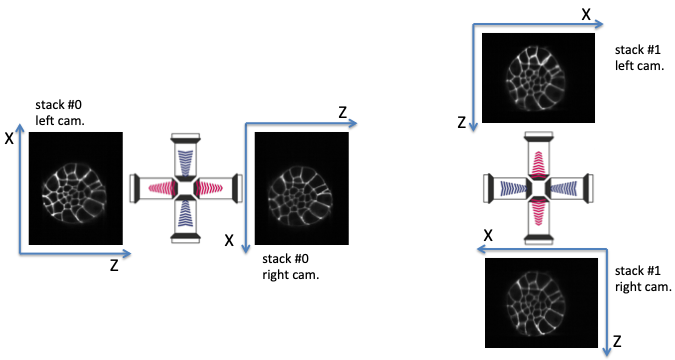
\includegraphics[width=150mm]{figures/acquisition-spim-right.png}
\end{center}
\caption{\label{fig:cli:fuse:spim:right:acquisition} Multiview lightsheet microscope acquisition: at a time point, two acquisitions (stack \#0 and stack \#1) are sequentially performed, the second one orthogonal to the first. For each acquisition, two 3D intensity image stacks are acquired, respectively by the left and the right cameras. 
It yields four image stacks to be fused. 
The frame $(\mathbf{X}, \mathbf{Z})$ of the left camera of stack \#0 needs to be rotated clockwise (90 degrees along the $\mathbf{Y}$ axis) to correspond to the frame of the left camera of stack \#1: \texttt{raw\_ori} has to be set to \texttt{'right'}.}
\end{figure}

\begin{figure}
\begin{center}
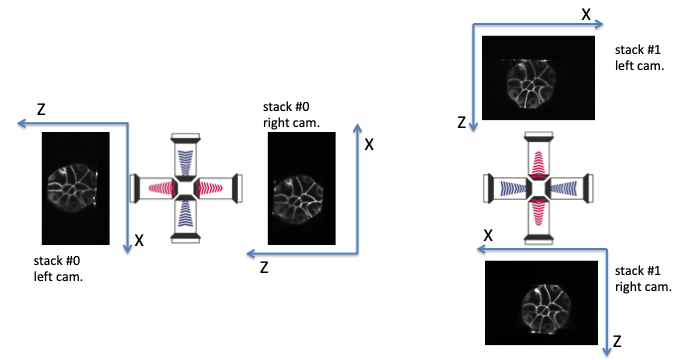
\includegraphics[width=150mm]{figures/acquisition-spim-left.png}
\end{center}
\caption{\label{fig:cli:fuse:spim:left:acquisition} The frame $(\mathbf{X}, \mathbf{Z})$ of the left camera of stack \#0 needs to be rotated counterclockwise (-90 degrees along the $\mathbf{Y}$ axis) to correspond to the frame of the left camera of stack \#1: \texttt{raw\_ori} has to be set to \texttt{'left'}.}
\end{figure}


\subsection{Important parameters in the parameter file}
\label{sec:cli:fuse:important:parameters}

A simple parameter file for fusion is described in the tutorial
section \ref{sec:tutorial:fusion}. A more comprehensive parameter file
example is provided in the \texttt{parameter-file-examples/} directory.

Indicating the right values of the
acquisition parameters is crucial; these parameters are
\begin{itemize}
\itemsep -1ex
\item \texttt{raw\_ori} is a parameter describing the acquisition
  orientation of the acquisition of the second pair of images. Its value can be either \texttt{'left'} (orientation of
  $270 \degree$) or \texttt{'right'} (orientation of
  $90 \degree$), see figures \ref{fig:cli:fuse:spim:right:acquisition} and \ref{fig:cli:fuse:spim:left:acquisition}.
\item \texttt{raw\_mirrors} is a parameter indicating whether the
  right camera images have been mirrored along the \textbf{X} axis or not. Its value is either \texttt{False} or \texttt{True}. For acquisitions depicted in figures \ref{fig:cli:fuse:spim:right:acquisition} and \ref{fig:cli:fuse:spim:left:acquisition}, it has to be set to \texttt{False}, meaning that the mirroring has to be done.
\item \texttt{raw\_resolution} is the voxel size (along the 3
    dimensions X, Y and Z) of the acquired images.
\item \texttt{target\_resolution} is the desired isotropic (the
    same along the 3 dimensions) voxel size for the result fusion
    images.
\item \texttt{begin} gives the index of the first time point to be
  processed.
\item \texttt{end} gives the index of the last time point to be processed.
\end{itemize}


When one may not be sure of the \texttt{raw\_ori} and
\texttt{raw\_mirrors} right values, it is advised to perform the
fusion on only one time point (by indicating the same index for both
\texttt{begin}  and \texttt{end}), with the four possibilities for the
variable couple (\texttt{raw\_ori}, \texttt{raw\_mirrors}), i.e.
(\texttt{'left'}, \texttt{False}),
(\texttt{'left'}, \texttt{True}),
(\texttt{'right'}, \texttt{False}), and
(\texttt{'right'}, \texttt{True}).
It comes to write four parameter files that differ only for the
parameters \texttt{raw\_ori}, \texttt{raw\_mirrors}, and
\texttt{EXP\_FUSE}  (to store the fusion result in different
directories, see section \ref{sec:cli:fuse:output:data}).
For these first experiments, it is also advised to set
\texttt{target\_resolution} to a large value, in order to speed up the
calculations.



\subsection{Input data}
\label{sec:cli:fuse:input:data}

Input data (acquired images from the MuViSPIM microscope) are assumed
to be organized in a separate \texttt{RAWDATA/} directory in the 
\texttt{/path/to/experiment/} directory as depicted below. 
\begin{itemize}
  \itemsep -1ex
\item \texttt{RAWDATA/LC/Stack000} contains the images acquired at the
  first angulation by the left camera.
\item \texttt{RAWDATA/LC/Stack001} contains the images acquired at the
  second angulation by the left camera.
\item \texttt{RAWDATA/RC/Stack000} contains the images acquired at the
  first angulation by the right camera.
\item \texttt{RAWDATA/RC/Stack001} contains the images acquired at the
  second angulation by the right camera.
\end{itemize}

\mbox{}
\dirtree{%
.1 /path/to/experiment/.
.2 RAWDATA/.
.3 LC/.
.4 Stack0000/.
.5 Time000xxx\_00.zip.
.5 {\ldots}.
.5 Time000xxx\_00.zip.
.4 Stack0001/.
.5 Time000xxx\_00.zip.
.5 {\ldots}.
.5 Time000xxx\_00.zip.
.3 RC/.
.4 Stack0000/.
.5 Time000xxx\_00.zip.
.5 {\ldots}.
.5 Time000xxx\_00.zip.
.4 Stack0001/.
.5 Time000xxx\_00.zip.
.5 {\ldots}.
.5 Time000xxx\_00.zip.
.2 \ldots.
}
\mbox{}

where \texttt{xxx} denotes a three digit number (e.g. $000$, $001$,
...) denoting the time point of each acquisition. The range of time
points to be fused are given by the variables \texttt{begin} and
\texttt{end}, while the path \texttt{/path/to/experiment/} has to be
assigned to the variable \texttt{PATH\_EMBRYO} 

Hence a parameter file containing
\begin{verbatim}
PATH_EMBRYO = /path/to/experiment/
begin = 0
end = 10
\end{verbatim}
indicates that time points in $[0,10]$ of the \texttt{RAWDATA/}
subdirectory of  \texttt{/path/to/experiment/} have to be fused.

\subsubsection{Input data directory names}

However, directories may be named differently. The variables
\texttt{DIR\_RAWDATA}, \texttt{DIR\_LEFTCAM\_STACKZERO},
\texttt{DIR\_RIGHTCAM\_STACKZERO}, \texttt{DIR\_LEFTCAM\_STACKONE},
and \texttt{DIR\_RIGHTCAM\_STACKONE} allow a finer control of the
directory names. The images acquired at the first angulation by the
left and the right cameras are searched in the directories
\begin{verbatim}
<PATH_EMBRYO>/<DIR_RAWDATA>/<DIR_LEFTCAM_STACKZERO>
<PATH_EMBRYO>/<DIR_RAWDATA>/<DIR_RIGHTCAM_STACKZERO>
\end{verbatim}
while the images acquired at the second angulation by the
left and the right cameras are searched in the directories
\begin{verbatim}
<PATH_EMBRYO>/<DIR_RAWDATA>/<DIR_LEFTCAM_STACKONE>
<PATH_EMBRYO>/<DIR_RAWDATA>/<DIR_RIGHTCAM_STACKONE>
\end{verbatim}
where \texttt{<XXX>} denotes the value of the variable \texttt{XXX}.
Then, to parse the following data architecture

\mbox{}
\dirtree{%
.1 /path/to/experiment/.
.2 my\_raw\_data/.
.3 LeftCamera/.
.4 FirstStack/.
.5 {\ldots}.
.4 SecondStack/.
.5 {\ldots}.
.3 RightCamera/.
.4 FirstStack/.
.5 {\ldots}.
.4 SecondStack/.
.5 {\ldots}.
.2 \ldots.
}
\mbox{}

one has to add the following lines in the parameter file
\begin{verbatim}
DIR_RAWDATA = 'my_raw_data'
DIR_LEFTCAM_STACKZERO = 'LeftCamera/FirstStack'
DIR_RIGHTCAM_STACKZERO = 'RightCamera/FirstStack'
DIR_LEFTCAM_STACKONE = 'LeftCamera/SecondStack'
DIR_RIGHTCAM_STACKONE = 'RightCamera/SecondStack'
\end{verbatim}

It has to be noted that, when the stacks of a given time point are in
different directories, image file names are tried to be guessed from
the directories parsing. It has to be pointed out that indexes have to
be encoded with a 3-digit integer with 0 padding (i.e. $000$, $001$,
\ldots) and that has to be the only variation in the file names
(within each directory).

\subsubsection{Input data image file names}

Images acquired from the left and the right cameras may be stored in
the same directory, but obviously with different names as in 

\mbox{}
\dirtree{%
.1 /path/to/experiment/.
.2 RAWDATA/.
.3 stack\_0\_channel\_0.
.4 Cam\_Left\_00xxx.zip.
.4  \ldots .
.4 Cam\_Right\_00xxx.zip.
.4 \ldots .
.3 stack\_1\_channel\_0.
.4 Cam\_Left\_00xxx.zip.
.4  \ldots .
.4 Cam\_Right\_00xxx.zip.
.4 \ldots .
}
\mbox{}

The parameter file has then to contain the following lines to indicate
the directory names.
\begin{verbatim}
DIR_LEFTCAM_STACKZERO = 'stack_0_channel_0'
DIR_RIGHTCAM_STACKZERO = 'stack_0_channel_0'
DIR_LEFTCAM_STACKONE = 'stack_1_channel_0'
DIR_RIGHTCAM_STACKONE = 'stack_1_channel_0'
\end{verbatim}

In addition, to distinguish the images acquired by the left camera to
those acquired by the right one, one has to give the image name
prefixes, i.e. the common part of the image file names before the
3-digit number that indicates the time point.
This is the purpose of the  variables
\verb|acquisition_leftcam_image_prefix| and 
\verb|acquisition_rightcam_image_prefix|.
The parameter file has then to contain the following lines not only to indicate
the directory names but also the image file name prefixes.

\begin{verbatim}
DIR_LEFTCAM_STACKZERO = 'stack_0_channel_0'
DIR_RIGHTCAM_STACKZERO = 'stack_0_channel_0'
DIR_LEFTCAM_STACKONE = 'stack_1_channel_0'
DIR_RIGHTCAM_STACKONE = 'stack_1_channel_0'
acquisition_leftcam_image_prefix = 'Cam_Left_00'
acquisition_rightcam_image_prefix = 'Cam_Right_00'
\end{verbatim}

\subsubsection{Multichannel acquisition}

In case of multichannel acquisition, the fusion is computed for the
first channel, and the computed parameters (e.g. transformations,
etc.) are also used for the other channels. 

For a second channel, 
the images acquired at the first angulation by the
left and the right cameras are searched in the directories
\begin{verbatim}
<PATH_EMBRYO>/<DIR_RAWDATA>/<DIR_LEFTCAM_STACKZERO_CHANNEL_2>
<PATH_EMBRYO>/<DIR_RAWDATA>/<DIR_RIGHTCAM_STACKZERO_CHANNEL_2>
\end{verbatim}
while the images acquired at the second angulation by the
left and the right cameras are searched in the directories
\begin{verbatim}
<PATH_EMBRYO>/<DIR_RAWDATA>/<DIR_LEFTCAM_STACKONE_CHANNEL_2>
<PATH_EMBRYO>/<DIR_RAWDATA>/<DIR_RIGHTCAM_STACKONE_CHANNEL_2>
\end{verbatim}

For a third channel, 
the images acquired at the first angulation by the
left and the right cameras are searched in the directories
\begin{verbatim}
<PATH_EMBRYO>/<DIR_RAWDATA>/<DIR_LEFTCAM_STACKZERO_CHANNEL_3>
<PATH_EMBRYO>/<DIR_RAWDATA>/<DIR_RIGHTCAM_STACKZERO_CHANNEL_3>
\end{verbatim}
while the images acquired at the second angulation by the
left and the right cameras are searched in the directories
\begin{verbatim}
<PATH_EMBRYO>/<DIR_RAWDATA>/<DIR_LEFTCAM_STACKONE_CHANNEL_3>
<PATH_EMBRYO>/<DIR_RAWDATA>/<DIR_RIGHTCAM_STACKONE_CHANNEL_3>
\end{verbatim}



\subsection{Output data}
\label{sec:cli:fuse:output:data}

The variable \texttt{target\_resolution} allows to set the desired isotropic (the
same along the 3 dimensions) voxel size for the result fusion
images.

\subsubsection{Output data directory names}

The resulting fused images are stored in sub-directory
\texttt{FUSE/FUSE\_<EXP\_FUSE>} under the
\texttt{/path/to/experiment/} directory 

\mbox{}
\dirtree{%
.1 /path/to/experiment/.
.2 RAWDATA/.
.3 \ldots.
.2 FUSE/.
.3 FUSE\_<EXP\_FUSE>/.
.4 \ldots.
}
\mbox{}

where \texttt{<EXP\_FUSE>} is the value of the variable \texttt{EXP\_FUSE} (its
default value is '\texttt{RELEASE}'). Hence, the line
\begin{verbatim}
EXP_FUSE = 'TEST'
\end{verbatim}
in the parameter file will create the directory
\texttt{FUSE/FUSE\_TEST/} in which the fused images are stored. For
instance, when testing for the values of the variable couple
(\texttt{raw\_ori}, \texttt{raw\_mirrors}), a first parameter file may
contain
\begin{verbatim}
raw_ori = 'left'
raw_mirrors = False
begin = 1
end = 1
EXP_FUSE=TEST-LEFT-FALSE
\end{verbatim}
a second parameter file may
contain
\begin{verbatim}
raw_ori = 'left'
raw_mirrors = True
begin = 1
end = 1
EXP_FUSE=TEST-LEFT-TRUE
\end{verbatim}
etc. The resulting fused images will then be in different directories

\mbox{}
\dirtree{%
.1 /path/to/experiment/.
.2 RAWDATA/.
.3 \ldots.
.2 FUSE/.
.3 FUSE\_TEST-LEFT-FALSE/.
.4 \ldots.
.3 FUSE\_TEST-LEFT-TRUE/.
.4 \ldots.
.3 \ldots.
}
\mbox{}

This will ease their visual inspection to decide which values of the variable couple
(\texttt{raw\_ori}, \texttt{raw\_mirrors}) to use for the fusion.

\subsubsection{Output data file names}

Fused image files are named after the variable \texttt{EN}:
\texttt{<EN>\_fuse\_t<xxx>.inr} where \texttt{<xxx>} is the time point
index encoded by a 3-digit integer (with 0 padding).


\subsubsection{Multichannel acquisition}

Variables \texttt{EXP\_FUSE\_CHANNEL\_2} and
\texttt{EXP\_FUSE\_CHANNEL\_3} allows to set the directory names for
the resulting fused images of the other channels.

\subsection{Fusion parameters}

% \subsubsection{Step \ref{it:fusion:slit:line}: slit line correction}

\subsubsection{Step \ref{it:fusion:crop:1}: raw data cropping}
\label{sec:cli:fuse:raw:data:cropping}

For computational cost purposes, raw data (images acquired by the MuViSPIM microscope) are cropped (only in X and Y dimensions) before co-registration. A threshold is computed with Otsu's method \cite{otsu:tsmc:1979} on the maximum intensity projection (MIP) image. The cropping parameters are computed to keep the above-threshold points in the MIP image, plus some extra margins. Hyper-intense areas may biased the threshold computation, hence the cropping.

To desactivate this cropping, the line
\begin{verbatim}
raw_crop = False
\end{verbatim}
has to be added in the parameter file.

\subsubsection{Step \ref{it:fusion:registration}: linear registration}
\label{sec:cli:fuse:linear:registration}

To decrease the computational cost, images are normalized and cast on one byte before registration. While it generally does not degrade the registration quality, it may induce troubles when hyper-intensities areas are present in the image. In such a case, the useful information may then be summarized in only a few intensity values.

Intensity normalization in registration can be deactivated by adding the following line in the parameter file
\begin{verbatim}
fusion_registration_normalization = False
\end{verbatim}

To verify whether a good quality registration can be conducted, the searched transformation type can be changed for a simpler one than affine. 
Adding the following line in the parameter file.
\begin{verbatim}
fusion_registration_transformation_type = translation
\end{verbatim}
will search for a translation which is supposed to be sufficient, according that only translations relates the 4 acquisitions of the MuViSPIM microscope (in a perfect setting). If the search for an affine transformation (the default behavior) failed (the fusion looks poor) while the search for a translation is successful (the fusion looks good), a two-steps registration may help to refine the found translation by a subsequent affine transformation as explained below.

Hyper-intensities areas may also bias the threshold calculation used for the automatic crop (step \ref{it:fusion:crop:1} of fusion). In such cases, the iterative registration method may find a local minimum that is not the desired one, because the relative positions of the two images to be co-registered are too far apart. To circumvent such a behavior, a two-steps registration can be done. It consists on a first pre-registration with a transformation with fewer degrees of freedom (i.e. a 3D translation). 

This pre-registration can be activated by adding the following line in the parameter file.
\begin{verbatim}
fusion_preregistration_compute_registration = True
\end{verbatim}
It may be also preferable to  deactivate the image normalization for both registration steps with
\begin{verbatim}
fusion_preregistration_normalization = False
fusion_registration_normalization = False
\end{verbatim}



\subsubsection{Step \ref{it:fusion:crop:2}: fused data cropping}
\label{sec:cli:fuse:fused:data:cropping}

To save disk storage, fused images are cropped at the end of the fusion stage. To desactivate this cropping, the line
\begin{verbatim}
fusion_crop = False
\end{verbatim}
has to be added in the parameter file.

\subsection{Troubleshooting}

\begin{itemize}
\item The fused images are obviously wrong.
  \begin{enumerate}
  \item Are the values of the variable couple (\texttt{raw\_ori}, \texttt{raw\_mirrors}) the right ones? Conduct experiments as suggested in section \ref{sec:cli:fuse:important:parameters}  (see also section \ref{sec:cli:fuse:output:data}) to get the right values.
  \item The registration may have failed.
    \begin{enumerate}
    \item Deactivate the 1-byte normalization (see section \ref{sec:cli:fuse:linear:registration}).
    \item Try to register with a simpler transformation type (i.e. translation) and/or with a two-steps registration (see section \ref{sec:cli:fuse:linear:registration}).
    \end{enumerate}
  \end{enumerate}
\item The imaged sample is cropped by the image border in the fused image.
  \begin{enumerate}
  \item Check whether the imaged sample was not already cropped in the raw data.
  \item The automated cropping may have failed. It is more likely to happen when cropping the raw data, so deactivate it (see section \ref{sec:cli:fuse:raw:data:cropping}). If it still happens, try to deactivate also the fused image cropping   (see section \ref{sec:cli:fuse:fused:data:cropping}).
  \end{enumerate}
\end{itemize}

\subsection{Parameter list}

Please also refer to the file
\texttt{parameter-file-examples/1-fuse-parameters.py}

\begin{itemize}
\itemsep -1ex
\item \texttt{DIR\_LEFTCAM\_STACKONE} see section \ref{sec:cli:fuse:input:data}
\item \texttt{DIR\_LEFTCAM\_STACKONE\_CHANNEL\_2} see section \ref{sec:cli:fuse:input:data}
\item \texttt{DIR\_LEFTCAM\_STACKONE\_CHANNEL\_3} see section \ref{sec:cli:fuse:input:data}
\item \texttt{DIR\_LEFTCAM\_STACKZERO} see section \ref{sec:cli:fuse:input:data}
\item \texttt{DIR\_LEFTCAM\_STACKZERO\_CHANNEL\_2} see section \ref{sec:cli:fuse:input:data}
\item \texttt{DIR\_LEFTCAM\_STACKZERO\_CHANNEL\_3} see section \ref{sec:cli:fuse:input:data}
\item \texttt{DIR\_RAWDATA} see section \ref{sec:cli:fuse:input:data}
\item \texttt{DIR\_RAWDATA\_CHANNEL\_2} see section \ref{sec:cli:fuse:input:data}
\item \texttt{DIR\_RAWDATA\_CHANNEL\_3} see section \ref{sec:cli:fuse:input:data}
\item \texttt{DIR\_RIGHTCAM\_STACKONE} see section \ref{sec:cli:fuse:input:data}
\item \texttt{DIR\_RIGHTCAM\_STACKONE\_CHANNEL\_2} see section \ref{sec:cli:fuse:input:data}
\item \texttt{DIR\_RIGHTCAM\_STACKONE\_CHANNEL\_3} see section \ref{sec:cli:fuse:input:data}
\item \texttt{DIR\_RIGHTCAM\_STACKZERO} see section \ref{sec:cli:fuse:input:data}
\item \texttt{DIR\_RIGHTCAM\_STACKZERO\_CHANNEL\_2} see section \ref{sec:cli:fuse:input:data}
\item \texttt{DIR\_RIGHTCAM\_STACKZERO\_CHANNEL\_3} see section \ref{sec:cli:fuse:input:data}
\item \texttt{EN} see section \ref{sec:cli:fuse:output:data}
\item \texttt{EXP\_FUSE} see section \ref{sec:cli:fuse:output:data}
\item \texttt{EXP\_FUSE\_CHANNEL\_2} see section \ref{sec:cli:fuse:output:data}
\item \texttt{EXP\_FUSE\_CHANNEL\_3} see section \ref{sec:cli:fuse:output:data}
\item \texttt{PATH\_EMBRYO} see section \ref{sec:cli:fuse:input:data}
\item \texttt{RESULT\_IMAGE\_SUFFIX\_FUSE}
\item \texttt{acquisition\_leftcam\_image\_prefix}  see section \ref{sec:cli:fuse:input:data}
\item \texttt{acquisition\_mirrors} same as \texttt{raw\_mirrors}
\item \texttt{acquisition\_orientation} same as \texttt{raw\_ori}
\item \texttt{acquisition\_resolution} same as \texttt{raw\_resolution}
\item \texttt{acquisition\_rightcam\_image\_prefix}  see section \ref{sec:cli:fuse:input:data}
\item \texttt{acquisition\_slit\_line\_correction}
\item \texttt{begin} see section \ref{sec:cli:fuse:important:parameters}
\item \texttt{default\_image\_suffix}
\item \texttt{delta}
\item \texttt{end} see section \ref{sec:cli:fuse:important:parameters}
\item \texttt{fusion\_crop} see section \ref{sec:cli:fuse:fused:data:cropping}
\item \texttt{fusion\_margin\_x\_0}
\item \texttt{fusion\_margin\_x\_1}
\item \texttt{fusion\_margin\_y\_0}
\item \texttt{fusion\_margin\_y\_1}
\item \texttt{fusion\_preregistration\_compute\_registration} see section \ref{sec:cli:fuse:linear:registration}
\item \texttt{fusion\_preregistration\_lts\_fraction}
\item \texttt{fusion\_preregistration\_normalization} see section \ref{sec:cli:fuse:linear:registration}
\item \texttt{fusion\_preregistration\_pyramid\_highest\_level}
\item \texttt{fusion\_preregistration\_pyramid\_lowest\_level}
\item \texttt{fusion\_preregistration\_transformation\_estimation\_type}
\item \texttt{fusion\_preregistration\_transformation\_type}
\item \texttt{fusion\_registration\_compute\_registration}
\item \texttt{fusion\_registration\_lts\_fraction}
\item \texttt{fusion\_registration\_normalization} see section \ref{sec:cli:fuse:linear:registration}
\item \texttt{fusion\_registration\_pyramid\_highest\_level}
\item \texttt{fusion\_registration\_pyramid\_lowest\_level}
\item \texttt{fusion\_registration\_transformation\_estimation\_type}
\item \texttt{fusion\_registration\_transformation\_type} see section \ref{sec:cli:fuse:linear:registration}
\item \texttt{raw\_crop} see section \ref{sec:cli:fuse:raw:data:cropping}
\item \texttt{raw\_delay}
\item \texttt{raw\_margin\_x\_0}
\item \texttt{raw\_margin\_x\_1}
\item \texttt{raw\_margin\_y\_0}
\item \texttt{raw\_margin\_y\_1}
\item \texttt{raw\_mirrors} see section \ref{sec:cli:fuse:important:parameters}
\item \texttt{raw\_ori} see section \ref{sec:cli:fuse:important:parameters}
\item \texttt{raw\_resolution} see section \ref{sec:cli:fuse:important:parameters}
\item \texttt{result\_image\_suffix}
\item \texttt{target\_resolution} see section \ref{sec:cli:fuse:output:data}
\end{itemize}


%%%%%%%%%%%%%%%%%%%%%%%%%%%%%%%%%%%%%%%%%%%%%%%%%%%%%%%%%%%%
%
% 1.5-intraregistration.py
%
%%%%%%%%%%%%%%%%%%%%%%%%%%%%%%%%%%%%%%%%%%%%%%%%%%%%%%%%%%%%

\section{\texttt{1.5-intraregistration.py}}
\label{sec:cli:intraregistration}

The sequence intra-registration procedure can be done either after the fusion step, or after the (post-)segmentation step. It aims at
\begin{itemize}
\itemsep -1ex
\item compensating for the eventual motion of the imaged sample with respect to the microscope
\item resampling the fusion and/or the segmentation images into a common frame/geometry, so they can better be compared, and
\item building 2D+t images made of 2D sections from either the  fusion
  and/or the segmentation images, so that the quality of the fusion
  and/of the tracking step can be visually assessed. 
\end{itemize}


The intra-registration procedure is made of the following steps:
\begin{enumerate}
\itemsep -1ex
\item Co-registration of pairs of successive fused images (section
  \ref{sec:cli:intraregistration:coregistration}). This yields the
  transformations $T_{t+1 \leftarrow t}$. Fused images are located in
  \verb|<EMBRYO>/FUSE/FUSE_<EXP_FUSE>|: the parameter \verb|EXP_FUSE|
  is either set in the parameter file or is set at
  \verb|RELEASE|. This step may be long. 

\item Composition of transformations issued from the co-registration
  step. This step computes the transformations $T_{ref \leftarrow
    t}$. towards a reference image \verb|ref| given by the parameter
  \verb|intra_registration_reference_index|. 

\item Computation of the \textit{template} image (section
  \ref{sec:cli:intraregistration:template}). This \textit{template}
  image dimension are computed so that the useful information of all
  resampled images fits into it. Useful information can be issued from
  either the fused sequence, the segmentation sequence or the
  post-segmentation sequence. It is indicated by the
  \verb|intra_registration_template_type| which value can be either
  \verb|'FUSION'|,  \verb|'SEGMENTATION'|, or
  \verb|'POST-SEGMENTATION'|. This step may be long. 

\item Resampling of either the fused or the segmentation images
  (section \ref{sec:cli:intraregistration:resampling}). Note that
  changing the parameters for this step will not require to re-compute
  the first steps. 

\item Extraction of 2D+t images from the resampled sequences (section
  \ref{sec:cli:intraregistration:movies}). Note that changing the
  parameters for this step (i.e. requiring extra movies) will not
  require to re-compute the first steps, with an eventual exception
  for the resampling step. 

\end{enumerate}



\subsection{\texttt{1.5-intraregistration.py} options}

The following options are available:
\begin{description}
  \itemsep -1ex
\item[\texttt{-h}] prints a help message
\item[\texttt{-p \underline{file}}] set the parameter file to be parsed
\item[\texttt{-e \underline{path}}] set the
  \texttt{\underline{path}} to the directory where the
  \texttt{RAWDATA/} directory is located
\item[\texttt{-k}] allows to keep the temporary files
\item[\texttt{-f}] forces execution, even if (temporary) result files
  are already existing
\item[\texttt{-v}] increases verboseness (both at console and in the
  log file)
\item[\texttt{-nv}] no verboseness
\item[\texttt{-d}]  increases debug information (in the
  log file)
\item[\texttt{-nd}] no debug information
\end{description}


\subsection{Output data}

The results are stored in sub-directories
\texttt{INTRAREG/INTRAREG\_<EXP\_INTRAREG>} under the
\texttt{/path/to/experiment/} directory where \texttt{<EXP\_INTRAREG>} is the value of the variable \texttt{EXP\_INTRAREG} (its
default value is '\texttt{RELEASE}'). 

\dirtree{%
.1 /path/to/experiment/.
.2 \ldots.
.2 INTRAREG/.
.3 INTRAREG\_<EXP\_INTRAREG>/.
.4 CO-TRSFS/.
.4 FUSE/.
.4 LOGS/.
.4 MOVIES/.
.4 [POST/].
.4 [SEG/].
.4 TRSFS\_t<begin>-<end>/.
.2 \ldots.
}


\texttt{INTRAREG/INTRAREG\_<EXP\_INTRAREG>/FUSE} contains the fused
images after resampling in a common geometry (i.e. all image have the
same X, Y and Z dimensions)

\dirtree{%
.1 /path/to/experiment/.
.2 \ldots.
.2 INTRAREG/.
.3 INTRAREG\_<EXP\_INTRAREG>/.
.4 \ldots.
.4 FUSE/.
.5 <EN>\_intrareg\_fuse\_t<xxx>.inr
.4 \ldots.
.2 \ldots.
}



\subsection{Co-registration parameters}
\label{sec:cli:intraregistration:coregistration}
Default registration parameters for the co-registration are set by:
\begin{verbatim}
# intra_registration_compute_registration = True
# intra_registration_transformation_type = 'rigid'
# intra_registration_transformation_estimation_type = 'wlts'
# intra_registration_lts_fraction = 0.55
# intra_registration_pyramid_highest_level = 6
# intra_registration_pyramid_lowest_level = 3
# intra_registration_normalization = True
\end{verbatim}
Computed transformations are stored in \verb|INTRAREG/INTRAREG_<EXP>/CO-TRSFS|.
It may be advised to set the pyramid lowest level value to some higher value to speed up the co-registrations (recall that all pairs of successive images will be co-registered, i.e.
\begin{verbatim}
intra_registration_pyramid_lowest_level = 4
\end{verbatim}


\subsection{Template building parameters}
\label{sec:cli:intraregistration:template}

\begin{verbatim}
# intra_registration_reference_index = None
# intra_registration_template_type = 'FUSION'
# intra_registration_template_threshold = None
# intra_registration_resolution = 0.6
# intra_registration_margin = None
\end{verbatim}

The \verb|intra_registration_reference_index| allows to choose the reference image (the one which remains still, i.e. is only displaced by a translation), by default it is the first image image of the series (associated to \verb|begin|).

Depending on \verb|intra_registration_template_type| (\verb|'FUSION'|, \verb|'SEGMENTATION'| or \verb|'POST-SEGMENTATION'|, the two latter assume obviously that the segmentation has been done), the \textit{template} image can be built either after the fusion or the segmentation images. If no threshold is given by \verb|intra_registration_template_threshold|, the built template will be large enough to include all the transformed fields of view (in this case, the template is the same whatever \verb|intra_registration_template_type| is). 

If a threshold is given, the built template will be large enough to
include all the transformed points above the threshold. E.g., the
background is labeled with either '1' or '0' in segmentation images,
then a threshold of '2' ensures that all the embryo cells will not be
cut by the resampling stage.  In this case, adding an additional
margin to the template could be a good idea for visualization
purpose. Last but not least, using a larger resolution than the
\verb|target_resolution| (the resolution of the fused images) allows
to decrease the resampled images volume. This can be achieved by
setting \verb|intra_registration_resolution| to a larger value than
the one of \verb|target_resolution| (default is 0.6).

Thus, building a \textit{template} image after the segmentation images can be done with
\begin{verbatim}
# intra_registration_reference_index = None
intra_registration_template_type = "SEGMENTATION"
intra_registration_template_threshold = 2
# intra_registration_resolution = 0.6
intra_registration_margin = 10
\end{verbatim}

Computed transformations from the \textit{template} image as well as the \textit{template} image itself are stored in \verb|INTRAREG/INTRAREG<EXP>/TRSFS_t<F>-<L>/| where \verb|<F>| and \verb|L| are the first and the last index of the series (specified by \verb|begin| and \verb|end| from the parameter file).

\subsubsection{Resampling fusion/segmentation images}
\label{sec:cli:intraregistration:resampling}
The resampled fusion and segmentation images will be stored respectively in \verb|INTRAREG/INTRAREG_<EXP>/FUSE|, \verb|INTRAREG/INTRAREG_<EXP>/SEG/| and \verb|INTRAREG/INTRAREG_<EXP>/POST/|. Resampling is done either if the following parameters are set to \verb|True| or if movies are requested to be computed.

\begin{verbatim}
# intra_registration_resample_fusion_images = True
# intra_registration_resample_segmentation_images = False
# intra_registration_resample_post_segmentation_images = False
\end{verbatim}

\subsection{2D+t movies}
\label{sec:cli:intraregistration:movies}
For either visual assessment or illustration purposes, 2D+t (i.e. 3D) images can be built from 2D sections extracted from the resampled temporal series. This is controlled by the following parameters:
\begin{verbatim}
# intra_registration_movie_fusion_images = True
# intra_registration_movie_segmentation_images = False
# intra_registration_movie_post_segmentation_images = False

# intra_registration_xy_movie_fusion_images = [];
# intra_registration_xz_movie_fusion_images = [];
# intra_registration_yz_movie_fusion_images = [];

# intra_registration_xy_movie_segmentation_images = [];
# intra_registration_xz_movie_segmentation_images = [];
# intra_registration_yz_movie_segmentation_images = [];

# intra_registration_xy_movie_post_segmentation_images = [];
# intra_registration_xz_movie_post_segmentation_images = [];
# intra_registration_yz_movie_post_segmentation_images = [];
\end{verbatim}

If \verb|intra_registration_movie_fusion_images| is set to \verb|True|, a movie is made with the  XY-section located at the middle of each resampled fusion image (recall that, after resampling, all images have the same geometry). Additional XY-movies can be done by specifying the wanted Z values in \verb|intra_registration_xy_movie_fusion_images|. E.g.
\begin{verbatim}
intra_registration_xy_movie_fusion_images = [100, 200];
\end{verbatim}
will build two movies with XY-sections located respectively at Z values of 100 and 200. The same stands for the other orientation and for the resampled segmentation images.

\subsection{Parameter list}

Please also refer to the file
\texttt{parameter-file-examples/1.5-intraregistration-parameters.py}

\begin{itemize}
\itemsep -1ex
\item \texttt{EN}
\item \texttt{EXP\_FUSE}
\item \texttt{EXP\_INTRAREG}
\item \texttt{EXP\_POST}
\item \texttt{EXP\_SEG}
\item \texttt{PATH\_EMBRYO}
\item \texttt{begin}
\item \texttt{default\_image\_suffix}
\item \texttt{delta}
\item \texttt{end}
\item \texttt{intra\_registration\_compute\_registration}
\item \texttt{intra\_registration\_lts\_fraction}
\item \texttt{intra\_registration\_margin}
\item \texttt{intra\_registration\_movie\_fusion\_images}
\item \texttt{intra\_registration\_movie\_post\_segmentation\_images}
\item \texttt{intra\_registration\_movie\_segmentation\_images}
\item \texttt{intra\_registration\_normalization}
\item \texttt{intra\_registration\_pyramid\_highest\_level}
\item \texttt{intra\_registration\_pyramid\_lowest\_level}
\item \texttt{intra\_registration\_reference\_index}
\item \texttt{intra\_registration\_resample\_fusion\_images}
\item \texttt{intra\_registration\_resample\_post\_segmentation\_images}
\item \texttt{intra\_registration\_resample\_segmentation\_images}
\item \texttt{intra\_registration\_resolution}
\item \texttt{intra\_registration\_sigma\_segmentation\_images}
\item \texttt{intra\_registration\_template\_threshold}
\item \texttt{intra\_registration\_template\_type}
\item \texttt{intra\_registration\_transformation\_estimation\_type}
\item \texttt{intra\_registration\_transformation\_type}
\item \texttt{intra\_registration\_xy\_movie\_fusion\_images}
\item \texttt{intra\_registration\_xy\_movie\_post\_segmentation\_images}
\item \texttt{intra\_registration\_xy\_movie\_segmentation\_images}
\item \texttt{intra\_registration\_xz\_movie\_fusion\_images}
\item \texttt{intra\_registration\_xz\_movie\_post\_segmentation\_images}
\item \texttt{intra\_registration\_xz\_movie\_segmentation\_images}
\item \texttt{intra\_registration\_yz\_movie\_fusion\_images}
\item \texttt{intra\_registration\_yz\_movie\_post\_segmentation\_images}
\item \texttt{intra\_registration\_yz\_movie\_segmentation\_images}
\item \texttt{result\_image\_suffix}
\end{itemize}


%%%%%%%%%%%%%%%%%%%%%%%%%%%%%%%%%%%%%%%%%%%%%%%%%%%%%%%%%%%%
%
% 2-mars.py
%
%%%%%%%%%%%%%%%%%%%%%%%%%%%%%%%%%%%%%%%%%%%%%%%%%%%%%%%%%%%%

\section{\texttt{2-mars.py}}
\label{sec:cli:mars}

The name \texttt{mars} comes from \cite{fernandez:hal-00521491} where \texttt{MARS} is the acronym of \textit{multiangle image acquisition, 3D reconstruction and cell segmentation}.

This method aims at producing a segmentation of a membrane cell image (e.g.  a fused image) into a segmention image. This segmentation image is a integer-valued image where each integer labeled an unique cell in the image. By convention, '1' is the background label, while cells have labels greater than 2. It is  is made of the following steps:
\begin{enumerate}
\itemsep -1ex
\item  Optionally, a transformation of the input image.
\item A seeded watershed.
\end{enumerate}


\subsection{\texttt{2-mars.py} options}

The following options are available:
\begin{description}
  \itemsep -1ex
\item[\texttt{-h}] prints a help message
\item[\texttt{-p \underline{file}}] set the parameter file to be parsed
\item[\texttt{-e \underline{path}}] set the
  \texttt{\underline{path}} to the directory where the
  \texttt{RAWDATA/} directory is located
\item[\texttt{-k}] allows to keep the temporary files
\item[\texttt{-f}] forces execution, even if (temporary) result files
  are already existing
\item[\texttt{-v}] increases verboseness (both at console and in the
  log file)
\item[\texttt{-nv}] no verboseness
\item[\texttt{-d}]  increases debug information (in the
  log file)
\item[\texttt{-nd}] no debug information
\end{description}



\subsection{Output data}

The results are stored in sub-directories
\texttt{SEG/SEG\_<EXP\_SEG>} under the
\texttt{/path/to/experiment/} directory where where \texttt{<EXP\_SEG>} is the value of the variable \texttt{EXP\_SEG} (its
default value is '\texttt{RELEASE}'). 

\dirtree{%
.1 /path/to/experiment/.
.2 \ldots.
.2 SEG/.
.3 SEG\_<EXP\_SEG>/.
.4 <EN>\_mars\_t<begin>.inr.
.4 LOGS/.
.4 RECONSTRUCTION/.
.2 \ldots.
}

\subsection{Segmentation parameters}


\subsubsection{Input image for watershed computation}

Before the watershed segmentation, the input image may be pre-processed. This pre-processing is controlled by the two variables.
\begin{itemize}
\itemsep -1ex
\item \texttt{mars\_intensity\_transformation} whose values are to be chosen in \texttt{None}, \texttt{'Identity'}, or \texttt{'Normalization\_to\_u8'}. Default is \texttt{'Identity'}.
\item \texttt{mars\_intensity\_enhancement} whose values are to be chosen in \texttt{None} or \texttt{GACE}. Default is \texttt{None}.
\end{itemize}
Each of these variables, if not \texttt{None}, induce a transformation of the input (i.e. fused) image. If both values are not known, the input image for the watershed is the result of the maximum operator over the two images.

\begin{itemize}
\itemsep -1ex
\item \texttt{mars\_intensity\_transformation = 'Identity'}: the input image is not transformed. 
  \item \texttt{mars\_intensity\_transformation = 'Normalization\_to\_u8'}: input images are usually encoded on 2 bytes. The choice transformed the input image in an 1-byte image by linearly mapping the input image values from $[I_{min}, I_{max}]$ to $[0, 255]$. $I_{min}$ and $I_{max}$ correspond respectively to the 1\% and to the 99\% percentiles of the input image cumulative histogram. Values below $I_{min}$ are set to $0$ while values above $I_{max}$ are set to $255$.
  \item \texttt{mars\_intensity\_enhancement = 'GACE'}: \texttt{GACE}
    stands for \textit{Global Automated Cell Extractor}. This is the
    method described in \cite{michelin:hal-00915000,michelin:tel-01451608}. It consists in
    \begin{enumerate}
    \itemsep -1ex
    \item  extracting a centerplane image of the membranes,
    \item  thresholding this centerplane image, and 
    \item  reconstruct the membranes through a tensor voting method.
    \end{enumerate}
\end{itemize}

If the input image is transformed before segmented, the transformed image is named \texttt{<EN>\_fuse\_t<begin>\_membrane.inr} and stored in the directory \texttt{SEG/SEG\_<EXP\_SEG>/RECONSTRUCTION/} if the value of the variable \texttt{mars\_keep\_reconstruction} is set to \texttt{True}.
\subsubsection{Seeded watershed}

The seed extraction is made of the following steps:
\begin{enumerate}
\itemsep -1ex
\item Gaussian smoothing of the input image, the gaussian standard deviation being given by the variable \texttt{watershed\_seed\_sigma}.
\item Extraction of the $h$-minima of the previous image, $h$  being given by the variable \texttt{watershed\_seed\_hmin}.
\item Hysteresis thresholding (and labeling)  of the $h$-minima image, with a high threshold equal to $h$ and and a low threshold equal to $1$. It then only selects the $h$-minima that have an actual depth of $h$.
\end{enumerate}
Given the seeds, the watershed is performed on the smoothed input image (gaussian standard deviation being given by the variable \texttt{watershed\_membrane\_sigma}).


\subsection{Parameter list}

Please also refer to the file
\texttt{parameter-file-examples/2-mars-parameters.py}

\begin{itemize}
\itemsep -1ex
\item \texttt{EN}
\item \texttt{EXP\_FUSE}
\item \texttt{EXP\_SEG}
\item \texttt{PATH\_EMBRYO}
\item \texttt{begin}
\item \texttt{default\_image\_suffix}
\item \texttt{delta}
\item \texttt{mars\_begin}
\item \texttt{mars\_end}
\item \texttt{mars\_hard\_threshold}
\item \texttt{mars\_intensity\_enhancement}
\item \texttt{mars\_intensity\_transformation}
\item \texttt{mars\_keep\_reconstruction}
\item \texttt{mars\_manual}
\item \texttt{mars\_manual\_sigma}
\item \texttt{mars\_sample}
\item \texttt{mars\_sensitivity}
\item \texttt{mars\_sigma\_TV}
\item \texttt{mars\_sigma\_membrane}
\item \texttt{result\_image\_suffix}
\item \texttt{watershed\_membrane\_sigma}
\item \texttt{watershed\_seed\_hmin}
\item \texttt{watershed\_seed\_sigma}
\end{itemize}

%%%%%%%%%%%%%%%%%%%%%%%%%%%%%%%%%%%%%%%%%%%%%%%%%%%%%%%%%%%%
%
%  3-manualcorrection.py
%
%%%%%%%%%%%%%%%%%%%%%%%%%%%%%%%%%%%%%%%%%%%%%%%%%%%%%%%%%%%%

\section{\texttt{3-manualcorrection.py}}
\label{sec:cli:manual:correction}

The seeded watershed is likely to produce segmentation errors, even with a careful choice of parameters. It is advised to set the parameters to favour over-segmentations insted of under-segmentations since the former are much more easier to correct, which is the purpose of \texttt{3-manualcorrection.py}.


\subsection{\texttt{3-manualcorrection.py} options}

The following options are available:
\begin{description}
 \itemsep -1ex
\item[\texttt{-h}] prints a help message
\item[\texttt{-p \underline{file}}] indicates the parameter file to be parsed
\item[\texttt{-e \underline{path}}] indicates the
  \texttt{\underline{path}} to the directory where the
  \texttt{RAWDATA/} directory is located
\item[\texttt{-k}] allows to keep the temporary files
\item[\texttt{-f}] forces execution, even if (temporary) result files
  are already existing
\item[\texttt{-v}] increases verboseness (both at console and in the
  log file)
\item[\texttt{-nv}] no verboseness
\item[\texttt{-d}]  increases debug information (in the
  log file)
\item[\texttt{-nd}] no debug information
\item[\texttt{-i \underline{input\_image}}] set the \texttt{\underline{input\_image}} file to be corrected. Allows to skip the automated naming of files.
  \item[\texttt{-o \underline{output\_image}}] set the resulting \texttt{\underline{ouput\_image}} file to be saved. Allows to skip the automated naming of files. 
\item[\texttt{-m \underline{mapping\_file}}] set the \texttt{\underline{mapping\_file}} to be used for the correction.
\item[\texttt{-nsc \underline{smallest\_cells}}] set the number of the smallest cells to be displayed after correction. The smallest cells are the most likely to be issued from an over-segmentation.
\item[\texttt{-nlc \underline{largest\_cells}}] set the number of the largest cells to be displayed after correction. The largest cells are the most likely to be issued from an under-segmentation.  
\end{description}



\subsection{Output data}

The results are stored in sub-directories
\texttt{SEG/SEG\_<EXP\_SEG>} under the
\texttt{/path/to/experiment/} directory where where \texttt{<EXP\_SEG>} is the value of the variable \texttt{EXP\_SEG} (its
default value is '\texttt{RELEASE}').
\texttt{<EN>\_seg\_t<begin>.inr} is the correction of the segmentation image \texttt{<EN>\_mars\_t<begin>.inr}.

\dirtree{%
.1 /path/to/experiment/.
.2 \ldots.
.2 SEG.
.3 SEG\_<EXP\_SEG>.
.4 <EN>\_mars\_t<begin>.inr.
.4 <EN>\_seg\_t<begin>.inr.
.4 LOGS/.
.4 RECONSTRUCTION/.
.2 \ldots.
}

\subsection{Segmentation correction parameters}

\texttt{3-manualcorrection.py} parses a correction file whose name is given by the variable \texttt{mancor\_mapping\_file}. The syntax of this file is very simple. Lines beginning with \texttt{\#} are ignored (and can be used to insert comments in the files). Non-empty lines should contain two numbers separated by a space, and \texttt{3-manualcorrection.py} will replace the first number by the second in the segmentation file.

E.g. a cell $c$ is recognized to be over-segmented, and then is represented by two labels, says 9 and 10. Thus the line
\begin{framed}
\begin{verbatim}
10 9
\end{verbatim}
\end{framed}
will replace all 10's by 9's in the segmentation image,  thus $c$ will only be represented by 9's after correction. See also the tutorial section \ref{sec:tutorial:manual:correction} for an other example.

\subsection{Parameter list}

Please also refer to the file
\texttt{parameter-file-examples/3-manualcorrection-parameters.py}

\begin{itemize}
\itemsep -1ex
\item \texttt{EN}
\item \texttt{EXP\_SEG}
\item \texttt{PATH\_EMBRYO}
\item \texttt{begin}
\item \texttt{default\_image\_suffix}
\item \texttt{delta}
\item \texttt{mancor\_input\_seg\_file}
\item \texttt{mancor\_mapping\_file}
\item \texttt{mancor\_output\_seg\_file}
\item \texttt{mars\_begin}
\item \texttt{mars\_end}
\item \texttt{result\_image\_suffix}
\end{itemize}